% Báo cáo ngắn phần AI xử lý ảnh, Nhóm 10. Dựng bằng build.ps1 (latexmk -xelatex).
\documentclass[a4paper,fontsize=12pt,parskip=false,numbers=noenddot,bibliography=totoc]{scrartcl}

\usepackage{fontspec}
\setmainfont{Times New Roman}
\usepackage{polyglossia}
\setmainlanguage{vietnamese}

\usepackage[top=2.5cm,bottom=2cm,left=3cm,right=2cm,footskip=1cm]{geometry}
\usepackage{setspace}
\setstretch{1.15}
\setlength{\parindent}{1.2em}
\setlength{\parskip}{0.1em}

\usepackage{graphicx}
\usepackage[table]{xcolor}
\usepackage{amsmath}
\usepackage{booktabs,tabularx,multirow,array}
\usepackage{placeins}
\usepackage{subcaption}
\usepackage[font=small,labelfont=bf,skip=4pt]{caption}
\usepackage{enumitem}
\setlist{nosep,leftmargin=1.4em}
\usepackage{tikz}
\usetikzlibrary{positioning,arrows.meta,shapes.geometric,calc,fit,backgrounds,decorations.pathreplacing,shadows}
\usepackage{tikz-3dplot}
\usepackage{pgfplots}
\pgfplotsset{compat=1.18}
\usepgfplotslibrary{groupplots,fillbetween}
\usepackage[hidelinks]{hyperref}

% ----- bảng màu chung cho mọi hình TikZ và pgfplots
\definecolor{cXanh}{HTML}{1F5A96}  % xanh dương đậm: dev, E1, luồng chính
\definecolor{cCam}{HTML}{E07B24}   % cam: test, tầng 1, cảnh báo
\definecolor{cLuc}{HTML}{2E8B57}   % lục: nhãn thật, đạt
\definecolor{cHong}{HTML}{C2397F}  % hồng: ám hồng, lỗi camera
\definecolor{cTim}{HTML}{6B4FA0}   % tím: E2, mạng NAFNet
\definecolor{cXam}{HTML}{5B6770}   % xám: mốc, chú thích
\definecolor{cVang}{HTML}{D8A51D}  % vàng đất: độ cao, tô nền phụ

\pgfplotsset{
  baocao/.style={
    tick label style={font=\scriptsize}, scaled ticks=false, /pgf/number format/fixed,
    label style={font=\small},
    legend style={font=\scriptsize,draw=none,fill=none},
    /pgf/number format/use comma,
    /pgf/number format/1000 sep={\,},
    axis line style={cXam},
    major tick style={cXam},
    ymajorgrids, grid style={cXam!20},
  },
}
\pgfplotsset{colormap={baocao}{rgb255=(31,90,150) rgb255=(107,79,160) rgb255=(194,57,127) rgb255=(224,123,36) rgb255=(216,165,29)}}

% ----- tiêu đề mục: Times đậm, không dùng font sans của KOMA
\setkomafont{disposition}{\normalfont\bfseries}
\setkomafont{section}{\normalfont\bfseries\large}
\setkomafont{subsection}{\normalfont\bfseries\normalsize}
\setkomafont{subsubsection}{\normalfont\bfseries\itshape\normalsize}
\RedeclareSectionCommand[beforeskip=1.1em,afterskip=0.5em]{section}
\RedeclareSectionCommand[beforeskip=0.8em,afterskip=0.35em]{subsection}
\setcounter{tocdepth}{2}
\captionsetup[subfigure]{font=footnotesize,skip=2pt}

\renewcommand{\topfraction}{0.92}\renewcommand{\bottomfraction}{0.8}
\renewcommand{\textfraction}{0.06}\renewcommand{\floatpagefraction}{0.8}
\setcounter{topnumber}{4}\setcounter{bottomnumber}{3}\setcounter{totalnumber}{6}
\setlength{\textfloatsep}{8pt plus 2pt minus 3pt}\setlength{\floatsep}{6pt plus 2pt}\setlength{\intextsep}{6pt plus 2pt}
\newcommand{\ci}[2]{[#1;\,#2]}
\newcommand{\so}[1]{#1}
\setlength{\emergencystretch}{2.5em}

\begin{document}

% Trang bìa theo mẫu PTIT (khung trang trí + logo lấy từ báo cáo PTTK của nhóm).
\begin{titlepage}
\thispagestyle{empty}
\begin{tikzpicture}[remember picture,overlay]
  \node[anchor=north west,inner sep=0] at ($(current page.north west)+(17.5mm,-19mm)$)
    {
\includegraphics[width=178mm,height=262mm]{fig/khung-bia.png}};
\end{tikzpicture}
\setstretch{1.15}
\vspace*{-0.2cm}
\begin{center}
{\large\bfseries HỌC VIỆN CÔNG NGHỆ BƯU CHÍNH VIỄN THÔNG\\[2pt]
KHOA TRÍ TUỆ NHÂN TẠO\par}
\vspace{2pt}
\rule{5.2cm}{0.6pt}

\vspace{1.3cm}

\includegraphics[width=3.4cm]{fig/logo-ptit.png}

\vspace{1.2cm}
{\LARGE\bfseries BÁO CÁO BÀI TẬP LỚN\\[4pt]
HỌC PHẦN XỬ LÝ ẢNH\par}

\vspace{1.1cm}
\begin{minipage}{13.2cm}
\centering\large\bfseries
Đề tài: ``Ảnh chất lượng thấp từ camera giá rẻ trên drone: làm rõ cho người xem và phát hiện người''
\end{minipage}

\vspace{1.0cm}
\begin{tabular}{@{}l@{\hspace{1.2em}}l@{\hspace{1.6em}}l@{}}
\textbf{Giảng viên:} & PGS.TS. Phạm Văn Cường & \\[3pt]
\textbf{Nhóm:} & Nhóm 10 & \\[3pt]
\textbf{Thành viên:} & Nguyễn Duy Nghĩa & B23DCCN600\\
 & Nguyễn Tự Kiên & B23DCCN465\\
 & Nguyễn Minh Toàn & B23DCCN832\\
 & Nguyễn Thành Trung & B23DCCN861\\
\end{tabular}

\vfill
{\large\bfseries Hà Nội, 11/2026\par}
\vspace*{0.4cm}
\end{center}
\end{titlepage}


\pagenumbering{arabic}
\setcounter{page}{1}

\section{Bài toán}\label{sec:bai-toan}

Drone S500 của nhóm mang một bo camera riêng: ESP32-S3 N16R8 với cảm biến OV3660, gắn nhìn thẳng xuống đất. Bo phát luồng MJPEG qua Mobile Hotspot của laptop, mỗi khung là một JPEG 640$\times$480 nén ở mức chất lượng 12. Ngoài bãi bay, luồng đạt 2 đến 9 khung/s. Mọi xử lý AI chạy trên laptop (RTX 4060 Laptop 8 GB) trong phần mềm điều khiển IOT-CV, vì bo ESP32-S3 chỉ đủ sức nén và gửi ảnh.

Từ cùng một khung gốc, đồ án phải cho ra hai thứ. Thứ nhất là nhận diện: hộp $[x_1,y_1,x_2,y_2]$ kèm độ tin cậy cho lớp người, để web cảnh báo người vận hành. Thứ hai là ảnh rõ: một khung cùng cỡ, dễ nhìn hơn cho người ngồi trước màn hình. Hai đầu ra tách nhau: nhận diện chạy trên khung gốc, ảnh rõ chỉ phục vụ mắt người (Hình~\ref{fig:pipeline}). Luật đặt từ đầu là điểm số chỉ chấm trên khung bay thật; ảnh tự sinh được dùng để huấn luyện, không dùng để kết luận. Bài toán dùng kiến thức nâng cao chất lượng ảnh, hệ màu, nén JPEG và nhận dạng của học phần~\cite{baigiang,gonzalez}.

\begin{figure}[!htbp]
\centering
\resizebox{\textwidth}{!}{% Đường đi của một khung trong IOT-CV với ba gói ONNX (results/.../iotcv/README.md §1, bảng t9)
\begin{tikzpicture}[
  font=\scriptsize, node distance=3.5mm and 4.5mm,
  khoi/.style={draw=#1, fill=#1!12, rounded corners=2pt, line width=0.8pt, align=center, minimum height=11mm, text width=19mm},
  mui/.style={-{Stealth[length=2.2mm]}, line width=0.9pt, cXam},
]
\node[khoi=cHong] (cam) {\textbf{Camera}\\ESP32-S3 N16R8\\+ OV3660\\JPEG 640$\times$480};
\node[khoi=cVang, right=of cam, text width=17mm] (wifi) {\textbf{Wi-Fi}\\MJPEG qua HTTP\\2 đến 9 khung/s};
\node[khoi=cXanh, right=of wifi, text width=19mm] (gcs) {\textbf{Laptop}\\ONNX Runtime\\CUDA, RTX 4060\\Laptop 8 GB};
\node[khoi=cCam, above right=2mm and 7mm of gcs.east, anchor=south west, text width=23mm] (det) {\textbf{Tầng 1}\\detector YOLO11s\\gói ONNX nhận diện};
\node[khoi=cTim, right=of det, text width=19mm] (ver) {\textbf{Tầng 2}\\verifier EffNet-B0\\cắt 96 px, $s\geq0{,}35$};
\node[khoi=cLuc, right=of ver, text width=15mm] (trk) {\textbf{Tầng 3}\\track IoU 0,3\\$k=n=1$};
\node[khoi=cXanh, below right=2mm and 7mm of gcs.east, anchor=north west, text width=46mm] (enh) {\textbf{Ảnh rõ trực tiếp}: gói ONNX làm rõ\\bộ lọc cổ điển, bật sẵn};
\node[draw=cXam, rounded corners=2pt, fill=cXam!8, align=center, text width=15mm, minimum height=11mm, right=5mm of enh] (web) {\textbf{Web}\\luồng ``Ảnh rõ''};
\node[draw=cXam, rounded corners=2pt, fill=cXam!8, align=center, text width=15mm, minimum height=11mm, above=2mm of trk] (canh) {\textbf{Web}\\cảnh báo người};
\draw[mui] (cam) -- (wifi);
\draw[mui] (wifi) -- (gcs);
\draw[mui] (gcs.east) -- ++(3mm,0) |- (det.west);
\draw[mui] (gcs.east) -- ++(3mm,0) |- (enh.west);
\draw[mui] (det) -- (ver);
\draw[mui] (ver) -- (trk);
\draw[mui] (trk) -- (canh);
\draw[mui] (enh) -- (web);
\end{tikzpicture}
}
\caption[Đường đi của một khung trong IOT-CV]{Đường đi của một khung trong IOT-CV. Ba tầng nhận diện chạy trên khung gốc; ``Ảnh rõ'' là nhánh riêng cho người xem và bật sẵn.}
\label{fig:pipeline}
\end{figure}

Nhóm đo lỗi của camera trên 1\,115 khung dev của chuyến bay ngày 02/11/2026 (bản ghi \texttt{20261102-100941}); khung test không tham gia phép đo. Bảng~\ref{tab:camera} liệt kê các lỗi chính, Hình~\ref{fig:loi-camera} cho thấy chúng trên khung thật. Lỗi nặng nhất là ám hồng: ISP nhân hệ số cân bằng trắng cho R và B lớn hơn G, nên ở vùng gần bão hoà kênh G dừng trước, đường bê tông và mái tôn sáng thành mảng hồng. Hồ sơ đo này là đầu vào của bộ làm xấu D2 và của bộ lọc cổ điển.

\begin{table}[!htbp]
\centering\footnotesize
\caption[Lỗi ảnh đo trên 1\,115 khung dev]{Lỗi ảnh đo trên 1\,115 khung dev (hồ sơ \texttt{ov3660-esp32s3-q12-20261102}, bản 1.2.0). Số là trung vị, ngoặc là p5 và p95.}
\label{tab:camera}
\begin{tabularx}{\textwidth}{@{}l X l@{}}
\toprule
Lỗi & Đại lượng đo & Giá trị \\
\midrule
Ám hồng vùng sáng & tỉ lệ điểm có $R-G>25$ và $B-G>25$; khung có $>0{,}5\,\%$ điểm hồng & 0,17\,\% (0; 3,3\,\%); 31\,\% số khung \\
Mù như sương & dark channel ô 15 px (thang 0 đến 255) & 143,7 (134,6; 152,1) \\
Vỡ khối JPEG & tỉ số biên khối $8\times8$; bảng DQT & 2,68 (2,15; 3,52); Annex K $\times$ 0,75, 4:2:2 \\
Tối góc & tỉ số sáng góc/tâm; tiêu cự khớp $\cos^4$ & 0,81 (0,62; 0,93); 1\,016 px \\
Dải tối mép trái & bề rộng dải & 14 px (13; 16) \\
Nhoè & $\sigma$ PSF Gauss khớp từ MTF50 & 0,76 px \\
\bottomrule
\end{tabularx}
\end{table}

\begin{figure}[!htbp]
\centering
\begin{subfigure}[b]{0.43\textwidth}\centering
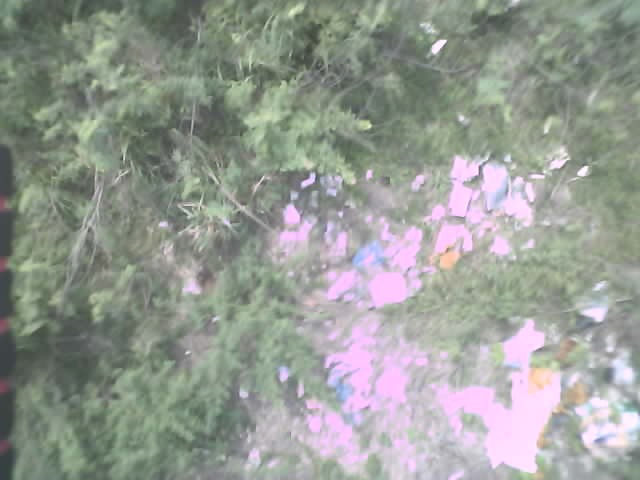
\includegraphics[width=\linewidth]{fig/art_full.jpg}
\caption{Khung \texttt{004\_01252}: mảng hồng, mù, tối góc}\end{subfigure}\hfill
\begin{subfigure}[b]{0.30\textwidth}\centering

\includegraphics[width=\linewidth]{fig/art_pink.jpg}
\caption{Mảng hồng phóng 4$\times$, thấy khối 8$\times$8}\end{subfigure}\hfill
\begin{subfigure}[b]{0.105\textwidth}\centering
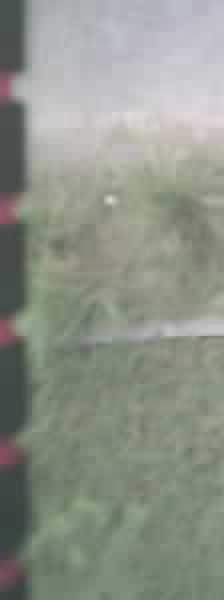
\includegraphics[width=\linewidth]{fig/art_strip.jpg}
\caption{Dải mép}\end{subfigure}\hfill
\begin{subfigure}[b]{0.13\textwidth}\centering

\includegraphics[width=\linewidth]{fig/art_block.jpg}
\caption{Biên khối, 8$\times$}\end{subfigure}
\caption[Lỗi của camera trên khung bay thật ngày 02/11/2026]{Lỗi của camera trên khung bay thật ngày 02/11/2026. Dải mép (c) rộng khoảng 14 cột nên mọi model bỏ 16 cột đầu.}
\label{fig:loi-camera}
\end{figure}

Một detector YOLO11s đứng một mình báo nhầm 0,881 hộp trên mỗi khung bay không người: túi rác, mảnh nhựa hồng, bóng người bị nhận thành người. Hệ của nhóm giải quyết hai chỗ: lọc báo nhầm bằng hai tầng đặt sau detector, và làm rõ ảnh bằng bộ lọc cổ điển chạy dưới dạng ONNX. Tập test 198 khung chỉ được chấm một lần, luật chọn ghi trước khi chạy.

\section{Dữ liệu}\label{sec:du-lieu}

\subsection{Khung bay thật, chia theo khối 30 giây}

Mọi khung thật đến từ sáu chuyến bay sáng 02/11/2026 trên cùng một bãi. Từ 17\,775 đoạn video, nhóm giữ khung nằm trong cửa sổ bay và cao trên 3 m, bỏ 29 khung có độ cao vọt bất thường, còn 2\,915 khung. Khung liền nhau của luồng 2 đến 9 khung/s gần như trùng nhau, nên chia ngẫu nhiên theo khung sẽ để ``anh em sinh đôi'' của khung test lọt vào tập huấn luyện. Nhóm cắt chuyến bay thành 24 khối 30 s, chọn 13 khối làm test theo tầng (độ cao, có người hay không), trong khối test chỉ lấy khung cách nhau ít nhất 1 s, và để vùng đệm 5 s quanh mỗi khối test.

Nhãn người của tập test được gán trước bằng nhiều model kèm SAHI, soát từng khung bằng mắt, rồi duyệt lần cuối trên Label Studio chạy tại máy; lượt duyệt cuối sửa 25,8\,\% số hộp. Phần dev được chia tiếp theo phiên bay (mỗi phiên là một chuyến): \texttt{devpool} để chọn model bằng k-fold theo phiên (fold 0 là phiên \#5, fold 1 là phiên \#1 đến \#4), \texttt{cal} gồm trọn hai khối dev để hiệu chỉnh ngưỡng, \texttt{mine} gồm khung không người để khai thác âm khó. Bảng~\ref{tab:split} tổng hợp các tập.

\begin{table}[!htbp]
\centering\footnotesize
\caption[Các tập dữ liệu]{Các tập dữ liệu. Ảnh ngoài đã qua lọc góc nhìn (nadir hoặc gần nadir); số trong ngoặc là ảnh có người.}
\label{tab:split}
\begin{tabularx}{\textwidth}{@{}l r X@{}}
\toprule
Tập & Khung / ảnh & Dùng để \\
\midrule
test (13 khối 30 s) & 198 & chấm một lần: 39 khung có người, 149 người, 159 khung bay không người \\
khung âm trong nhà (\texttt{neg}) & 300 & báo nhầm trong nhà, ba bản ghi khác \\
\texttt{devpool} & 160 & chọn model k-fold theo phiên: 70 khung có người, 218 người \\
\texttt{cal} (2 phiên, 16 khối) & 150 & hiệu chỉnh ngưỡng verifier và track; không người \\
\texttt{mine} & 85 & âm khó cho verifier; không người \\
\addlinespace
HERIDAL (CC BY 3.0) & 1\,684 (1\,086) & tập trộn \texttt{d02x}, mẫu dương và âm cho verifier \\
WiSARD (MIT) & 110 & \texttt{d02x}, mẫu dương và âm cho verifier \\
TinyPerson & 173 & chỉ làm mẫu dương cho verifier \\
VisDrone & 3\,493 cửa sổ & ảnh nguồn cho D0, D1, D2 (từ 1\,841 ảnh) \\
\bottomrule
\end{tabularx}
\end{table}

\subsection{Ảnh huấn luyện: dữ liệu ngoài và hai bộ làm xấu}

Khung bay thật có người quá ít để huấn luyện, nên ảnh huấn luyện lấy từ bộ ảnh drone có nhãn người. VisDrone~\cite{visdrone} là nguồn chính, cắt thành cửa sổ 624$\times$480 sao cho người có cỡ như trên khung thật. Nhóm thêm HERIDAL~\cite{heridal}, WiSARD~\cite{wisard} và TinyPerson~\cite{tinyperson}. Camera của nhóm nhìn thẳng xuống, nên ảnh ngoài phải qua lọc góc nhìn: một probe logistic trên đặc trưng CLIP, học từ nhãn VisDrone, giữ ảnh có điểm $\geq$ 0,8. Trên 100 ảnh soát tay mỗi bộ, probe chọn đúng 77/77 ảnh HERIDAL, 11/11 ảnh TinyPerson và 25/25 ảnh WiSARD (precision 1,00). HERIDAL chia train/val theo nơi bay (17 nơi) để không rò cảnh.

Ảnh nguồn sạch được làm xấu trước khi huấn luyện. D1 làm xấu ngẫu nhiên theo chuỗi bậc hai của Real-ESRGAN~\cite{realesrgan} và không đọc hồ sơ camera. D2 là bản sao camera: sáu khâu tất định theo thứ tự vật lý, từ không khí tới file JPEG (công thức ở mục~\ref{sec:suy-giam}). Khâu JPEG nén bằng đúng hai bảng lượng tử đọc từ file của camera, lấy mẫu màu 4:2:2; Pillow tái tạo được bảng và header của 20/20 khung dev thử.

Tham số D2 không đặt bằng tay. CMA-ES~\cite{cmaes} tìm 12 tham số sao cho thống kê của ảnh D2 sinh từ 500 ảnh nguồn cố định khớp 1\,115 khung dev. Hàm mục tiêu là trung bình 18 số hạng, mỗi số hạng là khoảng cách Wasserstein-1 giữa phân bố của một thống kê mức thấp (màu, dark channel, nhiễu, độ nét, khối JPEG, tối góc, phổ nhiễu) trên ảnh D2 và trên khung thật, chia cho IQR của khung thật:
\begin{equation}
\mathcal{L}(\theta)=\frac{1}{18}\sum_{j=1}^{18}\frac{W_1\!\big(F_j^{\mathrm{D2}(\theta)},\,F_j^{\mathrm{thật}}\big)}{\mathrm{IQR}_j}.
\label{eq:cmaes}
\end{equation}
Vòng 1 chạy 155 lượt, $\mathcal{L}$ giảm từ 0,967 xuống 0,736; vòng 2 nới các biên vòng 1 chạm, thêm tham số mức đen dư, chạy 80 lượt và xuống 0,712. Trên 198 khung test, khoảng cách thống kê của D2 là 0,80 so với 5,93 của D1 (mức sàn giữa hai nhóm khung thật là 0,33), và detector E1 học trên D2 báo nhầm 0,30 hộp/khung bay không người so với 0,99 của D1, hiệu $-0{,}692$ \ci{$-1{,}238$}{$-0{,}246$}. Tập \texttt{d02x} trộn VisDrone (D0 và D2) với HERIDAL và WiSARD, dùng cho thầy, trò và mẫu của verifier.

\section{Phương pháp}\label{sec:phuong-phap}

\subsection{Mô hình suy giảm D2}\label{sec:suy-giam}

D2 dựng lại chuỗi hỏng của camera theo đúng thứ tự vật lý. Gọi $J$ là ảnh nguồn sạch (thang 0 đến 1). Màn mờ theo mô hình khí quyển của He và cộng sự~\cite{he-dcp}, ống kính gồm nhoè Gauss và tối góc:
\begin{equation}
H = J\,t + A\,(1-t),\qquad L(\mathbf{x}) = V(\mathbf{x})\,\big(H * k_{\sigma}\big)(\mathbf{x}),\qquad V(\mathbf{x})=\Big(1+\tfrac{r(\mathbf{x})^2}{f^2}\Big)^{-2}=\cos^4\theta,
\label{eq:haze}
\end{equation}
với $A$ là airlight, $t$ chọn cho từng ảnh sao cho dark channel ra đúng một giá trị rút từ phân bố đo được, $r$ là khoảng cách tới tâm, $f$ là tiêu cự (hồ sơ đo 1\,016 px). Khâu tông màu nhân hệ số cân bằng trắng của ISP cho R và B (2,130 và 1,812 sau hiệu chỉnh) rồi cắt về miền hợp lệ; vì G bão hoà trước, điểm sáng rẽ khỏi trục xám về phía hồng. Sau đó là khâu ISP (làm mềm, nhiễu theo hàm mức nhiễu), dải tối mép trái 14 $\pm$ 1 px và JPEG bằng bảng lượng tử thật:
\begin{equation}
I_{\mathrm{D2}} = \mathcal{Q}_{\mathrm{q12}}\Big(\mathcal{E}\big(\mathcal{N}(\mathcal{T}(L))\big)\Big),
\label{eq:d2}
\end{equation}
trong đó $\mathcal{T}$ là tông màu, $\mathcal{N}$ là ISP và nhiễu, $\mathcal{E}$ là dải mép, $\mathcal{Q}_{\mathrm{q12}}$ là nén JPEG 4:2:2. Mười hai tham số của (\ref{eq:haze}) và (\ref{eq:d2}) được khớp bằng (\ref{eq:cmaes}).

\subsection{Nhận diện ba tầng}

\textit{Tầng 1, detector.} YOLO11s~\cite{yolo11} khởi từ COCO, tinh chỉnh trên D2 rồi tự huấn luyện trên khung dev chưa gán nhãn (E1 $\to$ E2), xuất ONNX opset 17 cho ONNX Runtime~\cite{onnxrt}. Graph nhận khung BGR \texttt{uint8} 480$\times$640$\times$3, cắt 16 cột, letterbox 1\,280, chạy mạng, NMS và trả hộp theo toạ độ khung gốc; ngưỡng vận hành 0,0767. Gói ONNX nhận diện kèm \texttt{meta.json} ghi sha256, ngưỡng và cấu hình track.

\textit{Tầng 2, verifier.} Một EfficientNet-B0~\cite{effnet} phân loại vùng cắt quanh từng hộp. Hộp $b$ được nới 1,5 lần, cạnh tối thiểu 32 px, cắt bằng RoiAlign ra 96$\times$96 ngay trong graph ONNX, nên phần mềm drone không phải tự cắt. Điểm và luật giữ hộp:
\begin{equation}
s(b)=\sigma\Big(g_{\phi}\big(\mathrm{RoiAlign}_{96}(I,\;1{,}5\,b)\big)\Big),\qquad \text{giữ } b \iff s(b)\geq\tau,\ \ \tau=0{,}35.
\label{eq:verifier}
\end{equation}
Mẫu huấn luyện có 18\,766 vùng cắt: 91 âm khó thật (hộp sai của detector trên \texttt{mine} và \texttt{devpool}), 1\,888 âm nền, 9\,444 hộp sai của detector trên ảnh \texttt{d02x}, cùng mẫu dương từ \texttt{devpool}, \texttt{d02x} và TinyPerson. Loss BCE có trọng số (âm khó thật $\times$4, dương thật $\times$3); mỗi vùng cắt được rung tâm $\pm$12\,\%, đổi cỡ $\pm$20\,\% và nén lại JPEG q25 đến q85 theo D2.

\textit{Tầng 3, lọc track.} Hộp ghép giữa các khung bằng IoU $\geq$ 0,3; một track chỉ báo khi có $k$ hộp trong $n$ khung. Tầng này cài một lần trong IOT-CV (mô-đun \texttt{track\_filter}); XLA hiệu chỉnh và chấm nó bằng cách gọi đúng mã đó.

\textit{Chọn điểm vận hành.} Luật D7, ghi trước, chỉ dùng \texttt{cal} và \texttt{devpool}: báo nhầm trên \texttt{cal} $\leq$ 0,03 hộp/khung, trong đó lấy recall \texttt{devpool} lớn nhất, hoà thì lấy cấu hình đơn giản nhất. Lưới 720 điểm (ngưỡng verifier 0 đến 0,95 $\times$ $k$ $\times$ $n$ $\times$ khoảng trống) chọn $\tau=0{,}35$ và $k=n=1$.

\subsection{Làm rõ ảnh: bộ lọc cổ điển chạy bằng ONNX}

Chuỗi lọc cổ điển (Hình~\ref{fig:classic}) đi ngược chuỗi hỏng của camera. Khử khối chạy trước tiên vì nó cần lưới 8$\times$8 còn nguyên: chỉ san bậc thang ở biên khối khi $|q_0-p_0|<\alpha=10$ và hai bên đều phẳng ($<\beta=4$). Khử hồng phải đứng trước khử mù, vì khử mù nhân sắc độ với $1/t$ làm loang vệt hồng: đặt sau chỉ xoá 46 đến 68\,\% điểm hồng, đặt trước xoá 93\,\%. Cổng hồng mở khi $\min(R,B)-G\geq6$ và $\max(R,B)\geq230$; mỗi lượt dịch sắc độ mà giữ độ sáng Y (BT.601):
\begin{equation}
\Delta=\lambda\,\alpha_m\Big(\tfrac{R+B}{2}-G\Big),\qquad R\leftarrow R-\Delta,\quad B\leftarrow B-\Delta,\quad G\leftarrow G+0{,}704\,\Delta,
\label{eq:magenta}
\end{equation}
với $\alpha_m$ là mặt nạ cổng đã nở 21 px và làm mềm, $\lambda=0{,}56$, hai lượt. Hệ số 0,704 = $(0{,}299+0{,}114)/0{,}587$ giữ Y không đổi. Bù tối góc chia cho $V(\mathbf{x})$ của (\ref{eq:haze}), trần 1,35. Khử mù đảo (\ref{eq:haze}) với dark channel ô 15 px~\cite{he-dcp}:
\begin{equation}
\tilde t(\mathbf{x}) = 1-\omega\,\frac{\mathrm{dark}(\mathbf{x})}{\overline{A}},\qquad t=\max\big(0{,}4,\ \mathrm{GF}(\tilde t)\big),\qquad J_c=\frac{I_c-A_c}{t}+A_c,
\label{eq:dehaze}
\end{equation}
với $\omega=0{,}85$ (giữ lại 15\,\% màn mờ), $A_c$ lấy theo từng kênh ở phân vị 99,9 của dark channel, GF là guided filter~\cite{guided} tính ở 1/4 độ phân giải. Cuối cùng làm nét unsharp trên Y, bỏ chi tiết $|d|\leq2\sigma_n$ để không làm nét nhiễu. Hình~\ref{fig:surf3d} cho thấy hai đại lượng mà chuỗi phải bù, đọc từ số đo thật.

\begin{figure}[!htbp]
\centering
% Chuỗi classic theo đúng thứ tự xla.enhance.classic.STEPS, tham số configs/enhance_classic.yaml 1.0.0
\begin{tikzpicture}[
  font=\scriptsize, x=1cm, y=1cm,
  buoc/.style={draw=#1, fill=#1!12, line width=0.8pt, rounded corners=2pt, align=center, text width=19mm, inner sep=1.5pt, minimum height=17mm},
  mui/.style={-{Stealth[length=1.8mm]}, line width=0.8pt, cXam},
]
\foreach \i/\ten/\mau/\ghi in {
  0/{Cắt 16 cột}/cXam/{bỏ dải mép},
  1/{Khử khối}/cCam/{chỉ trên lưới 8$\times$8,\\$\alpha$ 10, $\beta$ 4},
  2/{Khử hồng}/cHong/{$\min(R,B)-G\geq6$,\\$\max(R,B)\geq230$,\\giữ Y},
  3/{Bù tối góc}/cVang/{chia $\cos^4$,\\trần 1,35},
  4/{Khử mù}/cXanh/{dark channel 15 px,\\$\omega$ 0,85, $t\geq 0{,}4$},
  5/{Làm nét}/cLuc/{unsharp trên Y,\\bỏ $|d|\leq 2\sigma_n$},
  6/{Đệm mép}/cXam/{lặp cột 16}} {
  \node[buoc=\mau] (n\i) at (\i*2.28,0) {\textbf{\ten}\\[1pt]\ghi};
}
\foreach \i [evaluate=\i as \j using int(\i+1)] in {0,...,5} \draw[mui] (n\i) -- (n\j);
\node[anchor=north west, font=\scriptsize, cXam, text width=15.6cm] at ($(n0.west |- n2.south)+(0,-0.12)$) {Một graph ONNX opset 17, fp32, 703 nút; vào \texttt{frame} uint8 480$\times$640$\times$3 BGR, ra cùng cỡ. Sai khác với bản numpy trên 50 khung dev: MAE $\leq$ 0,018 (ORT CPU và CUDA).};
\end{tikzpicture}

\caption[Chuỗi lọc cổ điển trong gói ONNX làm rõ]{Chuỗi lọc cổ điển trong gói ONNX làm rõ (tham số \texttt{configs/enhance\_classic.yaml}).}
\label{fig:classic}
\end{figure}

\begin{figure}[!htbp]
\centering
% (a) hệ số tối góc cos^4 theo tiêu cự hồ sơ; (b) dark channel của một khung thật
\begin{subfigure}[b]{0.49\textwidth}\centering
\begin{tikzpicture}
\begin{axis}[baocao, ymajorgrids=false, width=7.0cm, height=5.6cm, view={-35}{32},
  xlabel={$x$ (px)}, ylabel={$y$ (px)}, zlabel={hệ số sáng},
  xmin=0,xmax=640,ymin=0,ymax=480,zmin=0.5,zmax=1.0,
  xtick={0,320,640}, ytick={0,240,480}, ztick={0.5,0.75,1},
  /pgf/number format/precision=2,
  colormap name=baocao, grid=major, grid style={cXam!15}]
\addplot3[surf, shader=interp, samples=26, samples y=20, domain=0:640, y domain=0:480, opacity=0.95]
  {1/(1+((x-320)^2+(y-240)^2)/1016.1^2)^2};
\addplot3[cHong, line width=1.2pt, samples=40, domain=0:640, samples y=1]
  (x,480,{1/(1+((x-320)^2+240^2)/690^2)^2});
\end{axis}
\end{tikzpicture}
\caption{Tối góc $\cos^4\theta$, $\tan\theta=r/f$, $f=1\,016$ px (hồ sơ). Đường hồng: mép dưới với $f=690$ px mà D2 dùng sau hiệu chỉnh.}
\label{fig:vignette3d}
\end{subfigure}\hfill
\begin{subfigure}[b]{0.49\textwidth}\centering
\begin{tikzpicture}
\begin{axis}[baocao, ymajorgrids=false, width=7.0cm, height=5.6cm, view={-35}{40},
  xlabel={$x$ (px)}, ylabel={$y$ (px)}, zlabel={dark channel},
  xmin=0,xmax=624,ymin=0,ymax=480,zmin=40,zmax=220, y dir=reverse,
  xtick={0,312,624}, ytick={0,240,480}, ztick={50,100,150,200},
  colormap name=baocao, grid=major, grid style={cXam!15}]
\addplot3[surf, shader=faceted interp, faceted color=black!25, line width=0.1pt]
  table[x=x,y=y,z=z] {fig/dark_channel.dat};
\end{axis}
\end{tikzpicture}
\caption{Dark channel (ô 15 px) của khung test \texttt{005\_00934}: trung vị 138, nền đường sáng lên tới 216.}
\label{fig:dc3d}
\end{subfigure}

\caption[Hai bề mặt 3D đọc từ số đo thật]{Hai bề mặt 3D đọc từ số đo thật: hệ số tối góc trên khung 640$\times$480 và dark channel của một khung bay. Dark channel cao khắp khung (gần 140/255): màn mờ phủ đều, gần cũng như xa, nên một $\overline{A}$ cho cả khung là đủ.}
\label{fig:surf3d}
\end{figure}

Viết bằng numpy/OpenCV, bộ lọc cổ điển nằm ngoài hợp đồng model của IOT-CV, nên nhóm dựng lại đúng năm tầng thành một graph ONNX: phép số nguyên của OpenCV thành phép float kèm \texttt{Round} và \texttt{Clip} đúng chỗ, \texttt{np.percentile} thành \texttt{TopK} cộng nội suy, nhánh \texttt{if} thành \texttt{Where}, erode/dilate thành \texttt{MaxPool}, lọc Gauss thành tổng lát dịch có trọng số. Graph không có \texttt{If}, \texttt{Loop}, \texttt{Conv} hay \texttt{MatMul}, nên không bị TF32 của ORT CUDA làm lệch phép làm tròn \texttt{uint8}.

Năm phương án học sâu được đo cùng thước để so: NAFNet-w16~\cite{nafnet} học ánh xạ D2 $\to$ D0, lai cổ điển $\to$ NAFNet, Real-ESRGAN x2plus~\cite{realesrgan} tinh chỉnh trên cặp D2 cho ảnh rõ offline sau chuyến bay, SwinIR-M x2~\cite{swinir} và BasicVSR++~\cite{basicvsrpp} cho video. Kết quả so ở Bảng~\ref{tab:sosanh}.

\subsection{Thước đo}

\textit{mAP50 và báo nhầm.} AP của lớp người là diện tích dưới đường precision theo recall khi hộp dự đoán khớp nhãn với IoU $\geq$ 0,5:
\begin{equation}
\mathrm{AP}_{50}=\int_0^1 p_{50}(r)\,dr,\qquad \mathrm{IoU}(b,g)=\frac{|b\cap g|}{|b\cup g|}.
\label{eq:map}
\end{equation}
Báo nhầm là số hộp sai trên mỗi khung bay không người. Mọi khoảng tin cậy 95\,\% lấy bằng bootstrap 2\,000 lần theo khối 30 s: rút lại khối chứ không rút khung lẻ, vì khung trong một khối tương quan và rút khung lẻ cho CI hẹp giả. Hai hệ được so bằng hiệu ghép cặp trên cùng mẫu bootstrap; một cải thiện được tính khi CI của hiệu không chạm 0.

\textit{Thử mù A/B.} Ảnh rõ không có đáp án trên khung thật, nên người xem là thước đo. Trang HTML chạy offline hiện hai ảnh cạnh nhau, trái phải xáo trộn, tên file là mã hex; người chấm chọn ảnh dễ nhìn hơn. Mỗi so sánh có $n=25$ cặp trên khung dev có người (không dùng khung test), thêm 5 cặp lặp đổi bên. Với $x$ lượt thắng, $\hat p=x/n$, $z=1{,}96$, khoảng Wilson~\cite{wilson} là
\begin{equation}
\frac{\hat p+\frac{z^2}{2n}\pm z\sqrt{\frac{\hat p(1-\hat p)}{n}+\frac{z^2}{4n^2}}}{1+\frac{z^2}{n}},
\label{eq:wilson}
\end{equation}
và một so sánh được tính là thắng khi cận dưới $>0{,}5$, tức từ 18/25. Luật chốt trước khi chấm: ảnh rõ offline chỉ được đưa vào phần mềm khi thắng cả ảnh gốc lẫn bộ lọc cổ điển ở lượt cả khung.

\section{Kết quả}\label{sec:ket-qua}

\subsection{Nhận diện: tầng xác minh cắt hai phần ba báo nhầm}

Bảng~\ref{tab:tang} và Hình~\ref{fig:tang} là kết quả chấm một lần trên 198 khung test, qua đúng đường IOT-CV chạy: phát lại bản ghi, ghi CSV từng tầng, chấm bằng \texttt{xla.eval.detection}. So YOLO11s một tầng với YOLO11s + verifier EfficientNet-B0 + lọc track (ba tầng) trên cùng 198 khung: mAP50 tăng từ 0,120 lên 0,210, hiệu $+0{,}090$ \ci{$+0{,}026$}{$+0{,}189$}, và báo nhầm trên khung bay không người giảm từ 0,881 xuống 0,289 hộp/khung, hiệu $-0{,}591$ \ci{$-1{,}033$}{$-0{,}273$}. Cả hai CI không chạm 0. Recall ở ngưỡng vận hành giữ nguyên 0,396 (59/149 người): verifier không bỏ người nào mà detector đã bắt được. Trên 300 khung trong nhà, báo nhầm ở mức 0,003 hộp/khung.

\begin{table}[!htbp]
\centering\footnotesize
\caption[Ba tầng nhận diện trên 198 khung test thật]{Ba tầng nhận diện trên 198 khung test thật (39 khung có người, 149 người). CI 95\,\% bootstrap theo khối 30 s. Báo nhầm tính trên 159 khung bay không người và 300 khung trong nhà.}
\label{tab:tang}
\setlength{\tabcolsep}{3.5pt}
\begin{tabular}{@{}l c c c c c@{}}
\toprule
Tầng & mAP50 [CI 95\,\%] & Recall & Báo nhầm, bay [CI 95\,\%] & Trong nhà & Ngưỡng \\
\midrule
1 detector & 0,119 \ci{0,032}{0,197} & 0,396 & 0,874 \ci{0,333}{1,486} & 0,003 & 0,077 \\
2 + verifier & 0,210 \ci{0,122}{0,312} & 0,396 & 0,289 \ci{0,036}{0,631} & 0,003 & 0,350 \\
3 + track $k1/n1$ & 0,210 \ci{0,122}{0,312} & 0,396 & 0,289 \ci{0,036}{0,631} & 0,003 & 0,350 \\
\midrule
ba tầng $-$ một tầng & $+0{,}090$ \ci{$+0{,}026$}{$+0{,}189$} & $+0{,}000$ & $-0{,}591$ \ci{$-1{,}033$}{$-0{,}273$} & & \\
\bottomrule
\end{tabular}
\end{table}

\begin{figure}[!htbp]
\centering
% Ba tầng trên 198 khung test (bảng t7, system/score.json). Thanh lỗi: CI 95 % bootstrap theo khối 30 s.
\begin{subfigure}[b]{0.49\textwidth}\centering
\begin{tikzpicture}
\begin{axis}[baocao, width=7.2cm, height=5.0cm, ybar, bar width=16pt,
  ymin=0, ymax=0.40, ylabel={mAP50 test}, xmin=0.4, xmax=3.6, xtick={1,2,3},
  xticklabels={{tầng 1\\detector},{tầng 2\\+ verifier},{tầng 3\\+ track}},
  x tick label style={align=center,font=\scriptsize}, /pgf/number format/precision=2,
  error bars/y dir=both, error bars/y explicit, error bars/error bar style={line width=0.7pt,black!70},
  error bars/error mark options={rotate=90,mark size=3pt,black!70}]
\addplot[fill=cCam, draw=none, bar shift=0pt] coordinates {(1,0.119) += (0,0.078) -= (0,0.087)};
\addplot[fill=cTim!85, draw=none, bar shift=0pt] coordinates {(2,0.210) += (0,0.102) -= (0,0.088)};
\addplot[fill=cLuc!85, draw=none, bar shift=0pt] coordinates {(3,0.210) += (0,0.102) -= (0,0.088)};
\node[font=\scriptsize, anchor=south] at (axis cs:1,0.205) {0,119};
\node[font=\scriptsize, anchor=south] at (axis cs:2,0.320) {0,210};
\node[font=\scriptsize, anchor=south] at (axis cs:3,0.320) {0,210};
\end{axis}
\end{tikzpicture}
\caption{mAP50 trên 198 khung test}
\label{fig:tang-map}
\end{subfigure}\hfill
\begin{subfigure}[b]{0.49\textwidth}\centering
\begin{tikzpicture}
\begin{axis}[baocao, width=7.2cm, height=5.0cm, ybar, bar width=16pt,
  ymin=0, ymax=1.75, ylabel={hộp sai / khung bay trống}, xmin=0.4, xmax=3.6, xtick={1,2,3},
  xticklabels={{tầng 1\\detector},{tầng 2\\+ verifier},{tầng 3\\+ track}},
  x tick label style={align=center,font=\scriptsize}, /pgf/number format/precision=2,
  error bars/y dir=both, error bars/y explicit, error bars/error bar style={line width=0.7pt,black!70},
  error bars/error mark options={rotate=90,mark size=3pt,black!70}]
\addplot[fill=cCam, draw=none, bar shift=0pt] coordinates {(1,0.874) += (0,0.612) -= (0,0.541)};
\addplot[fill=cTim!85, draw=none, bar shift=0pt] coordinates {(2,0.289) += (0,0.342) -= (0,0.253)};
\addplot[fill=cLuc!85, draw=none, bar shift=0pt] coordinates {(3,0.289) += (0,0.342) -= (0,0.253)};
\node[font=\scriptsize, anchor=south] at (axis cs:1,1.50) {0,874};
\node[font=\scriptsize, anchor=south] at (axis cs:2,0.64) {0,289};
\node[font=\scriptsize, anchor=south] at (axis cs:3,0.64) {0,289};
\end{axis}
\end{tikzpicture}
\caption{Báo nhầm trên 159 khung bay không người}
\label{fig:tang-fp}
\end{subfigure}

\caption[Ba tầng nhận diện trên 198 khung test]{Ba tầng nhận diện trên 198 khung test, thanh lỗi là CI 95\,\% bootstrap theo khối. Phần tăng mAP50 và phần giảm báo nhầm đều đến từ tầng 2.}
\label{fig:tang}
\end{figure}

Tầng 1 chạy qua IOT-CV cho đúng kết quả của detector chấm bằng XLA (hiệu mAP50 bằng 0, lệch một hộp báo nhầm trên 159 khung), nên phần chênh ở tầng 2 là của verifier. Trên \texttt{cal}, verifier ở $\tau=0{,}35$ bỏ 13/15 hộp sai; trên \texttt{devpool} (dự đoán ngoài fold) nó bỏ 25/79 hộp sai mà vẫn giữ đủ 58/218 người. Tầng 3 ở $k=1$ trùng tầng 2 từng hộp, đúng như luật D7 chọn: lọc track $k\geq2$ bỏ nốt 2 hộp sai trên \texttt{cal} nhưng mất ít nhất 10 người trên \texttt{devpool}. Ba gói ONNX (nhận diện, xác minh, làm rõ) đều qua kiểm golden của IOT-CV trên cả CUDA và CPU (detector IoU $\geq$ 0,9998, verifier lệch điểm $\leq$ 0,0003, bộ lọc cổ điển lệch $\leq$ 2 mức).

\subsection{Làm rõ ảnh: bộ lọc cổ điển thắng ảnh gốc 25/25}

Trên 198 khung test, bộ lọc cổ điển ONNX hạ tỉ lệ điểm hồng từ 0,943\,\% xuống 0,102\,\% (giảm 89,2\,\%) và hạ dark channel trung vị từ 139,0 xuống 56,5 (giảm 59,4\,\%); trên 50 khung dev các số tương ứng là 91,4\,\% và 60,4\,\%, nên dev và test không lệch nhau. Hình~\ref{fig:enh} là hai khung bay thật trước và sau: lớp sương xám được gỡ, cỏ về màu xanh, vệt hồng trên đường đất nhạt đi, người và bóng người nổi rõ khỏi nền.

\begin{figure}[!htbp]
\centering
\foreach \i/\c in {0/{\texttt{002\_00428}},2/{\texttt{007\_00765}}}{%
\begin{subfigure}[b]{0.285\textwidth}\centering\includegraphics[width=\linewidth]{fig/anh\i_raw.jpg}\caption*{gốc, \c}\end{subfigure}\hfill
\begin{subfigure}[b]{0.285\textwidth}\centering\includegraphics[width=\linewidth]{fig/anh\i_classic.jpg}\caption*{cổ điển ONNX}\end{subfigure}\hfill
\begin{subfigure}[b]{0.205\textwidth}\centering\includegraphics[width=\linewidth]{fig/anh\i_raw_zoom.jpg}\caption*{gốc, 2$\times$}\end{subfigure}\hfill
\begin{subfigure}[b]{0.205\textwidth}\centering\includegraphics[width=\linewidth]{fig/anh\i_classic_zoom.jpg}\caption*{cổ điển, 2$\times$}\end{subfigure}\par\smallskip}
\caption[Khung bay thật qua bộ lọc cổ điển ONNX]{Khung bay thật ngày 02/11 qua bộ lọc cổ điển ONNX: ảnh ra là đầu ra ORT đã lưu làm golden của gói ONNX làm rõ. Hai cột phải phóng 2$\times$ vùng có người (góc trên trái).}
\label{fig:enh}
\end{figure}

Bảng~\ref{tab:sosanh} đặt bộ lọc cổ điển cạnh các phương án đã đo. Ở thử mù A/B lượt cả khung (Hình~\ref{fig:ab}), bộ lọc cổ điển thắng ảnh gốc 25/25, Wilson \ci{0,867}{1,000}; năm cặp lặp đổi bên đều được chọn như lần đầu. Real-ESRGAN x2 tinh chỉnh cũng thắng ảnh gốc 25/25, còn khi đặt cạnh bộ lọc cổ điển nó được chọn 16/25, Wilson \ci{0,445}{0,798}: người chấm không phân biệt được hai cách ở cỡ cả khung. Hàng rào báo nhầm của ảnh offline qua (detector trên 150 khung \texttt{cal}: 15 hộp ở ảnh gốc, 10 hộp ở ảnh offline, hiệu $-0{,}033$ \ci{$-0{,}123$}{$+0{,}039$}).

\begin{table}[!htbp]
\centering\footnotesize
\caption[So sánh các phương pháp làm rõ ảnh]{So sánh các phương pháp làm rõ ảnh. Thời gian đo trên RTX 4060 Laptop, ONNX Runtime 1.24.4 trừ khi ghi khác; ``chuyến'' là một chuyến bay 20 phút (6\,750 khung ở 5,62 khung/s).}
\label{tab:sosanh}
\begin{tabularx}{\textwidth}{@{}>{\raggedright\arraybackslash}p{2.7cm} >{\raggedright\arraybackslash}p{3.3cm} >{\raggedright\arraybackslash}p{3.0cm} X@{}}
\toprule
Phương pháp & Kết quả đo & Tốc độ & Lý do chọn hay không chọn \\
\midrule
Bộ lọc cổ điển ONNX & A/B thắng gốc 25/25; hồng $-$89,2\,\%, dark channel $-$59,4\,\% (test) & 19,3 / 25,3 ms p50/p95 CUDA; 29,3 / 30,6 ms CPU & chọn, bật sẵn: không học nên không mang thiên lệch của ảnh huấn luyện, khử mù theo chính khung đang xem \\
\addlinespace
NAFNet-w16 & dark channel $-$36,8\,\%, màu ra nguội & 20,61 / 27,89 ms (cùng lượt đo) & không chọn: khử mù yếu hơn, chậm hơn 2,55 ms p95 \\
\addlinespace
Lai cổ điển $\to$ NAFNet & hết hồng; dark channel trung vị 84,0 đến 111,5 (cổ điển 56,0), dev & 7\,600 bước, 25 phút GPU & không xuất: mạng học theo đích VisDrone sạch nên trả lại màn mờ bộ lọc đã gỡ \\
\addlinespace
Real-ESRGAN x2 tinh chỉnh (offline) & A/B thắng gốc 25/25; với cổ điển 16/25 & 0,404 s/khung, 0,758 giờ GPU/chuyến & không chọn: A/B cả khung không phân biệt được với cổ điển, trong khi chậm hơn khoảng 20 lần \\
\addlinespace
SwinIR-M x2 & & 2,70 s/khung PyTorch; 17,4 s ORT & dừng ở bench: một chuyến cần 32,6 giờ GPU \\
\addlinespace
BasicVSR++ (5 khung) & & 3,34 s/khung PyTorch & dừng ở probe: ORT 1.24.4 không có kernel \texttt{DeformConv} \\
\bottomrule
\end{tabularx}
\end{table}

\subsection{Chạy trong phần mềm drone}

IOT-CV nạp ba gói ONNX và phát lại 600 khung của chuyến 02/11 (khung 284 đến 884) đúng nhịp thật, so hai cấu hình trong một tiến trình, bốn lượt xen kẽ ABBA: nhận diện một tầng + NAFNet (A) và ba tầng + bộ lọc cổ điển (B). Ở luồng mặc định có người xem ``Ảnh rõ'', p95 tổng của B là 89,5 ms so với 99,1 ms của A (p50 76,3 so với 84,5 ms), và tỉ lệ khung bị bỏ là 4,2 và 4,7\,\% so với 7,8 và 8,2\,\% (Hình~\ref{fig:ms}). Bộ lọc cổ điển nhẹ hơn NAFNet khoảng 15 ms p95 (19,3 so với 34,4 ms), đủ bù phần verifier thêm vào (p95 khoảng 9 ms, p50 0,03 ms vì phần lớn khung không có hộp qua tầng 1). Lệch giữa hai lượt cùng cấu hình $\leq$ 3,4 ms, nhỏ hơn chênh giữa hai cấu hình. GPU lúc đo chạy ở xung trung vị 780 đến 802 MHz (tối đa 3\,105), 70 đến 72\,\textdegree C; số tuyệt đối ghi kèm điều kiện này, hai cấu hình đo cùng điều kiện.

\begin{figure}[!htbp]
\centering
% (a) A/B mù, lượt cả khung (bảng t8); (b) p95 ms nhịp thật có "Ảnh rõ" (bảng t9)
\begin{subfigure}[b]{0.47\textwidth}\centering
\begin{tikzpicture}
\begin{axis}[baocao, width=6.1cm, height=4.9cm, xbar, /pgf/bar width=12pt,
  ymajorgrids=false, xmajorgrids, xmin=0, xmax=1.18, xlabel={tỉ lệ lượt bên thứ nhất thắng},
  xtick={0,0.25,0.5,0.75,1},
  ymin=0.4, ymax=3.6, ytick={1,2,3},
  yticklabels={{Real-ESRGAN $\times$2\\vs cổ điển},{Real-ESRGAN $\times$2\\vs gốc},{cổ điển\\vs gốc}},
  y tick label style={align=right,font=\scriptsize}, /pgf/number format/precision=2,
  error bars/x dir=both, error bars/x explicit, error bars/error bar style={line width=0.7pt,black!70},
  error bars/error mark options={mark size=3pt,black!70}]
\addplot[fill=cXanh!85, draw=none, bar shift=0pt] coordinates {(1.0,3) -= (0.133,0)};
\addplot[fill=cTim!80, draw=none, bar shift=0pt] coordinates {(1.0,2) -= (0.133,0) (0.64,1) += (0.158,0) -= (0.195,0)};
\draw[cXam, dashed] (axis cs:0.5,0.4) -- (axis cs:0.5,3.6);
\node[font=\scriptsize, anchor=west, white] at (axis cs:0.02,3) {25/25};
\node[font=\scriptsize, anchor=west, white] at (axis cs:0.02,2) {25/25};
\node[font=\scriptsize, anchor=west, white] at (axis cs:0.02,1) {16/25};
\end{axis}
\end{tikzpicture}
\caption{Thử mù A/B, 25 cặp mỗi so sánh, CI Wilson 95\,\%}
\label{fig:ab}
\end{subfigure}\hfill
\begin{subfigure}[b]{0.5\textwidth}\centering
\begin{tikzpicture}
\begin{axis}[baocao, width=7.4cm, height=4.9cm, ybar=1pt, bar width=9pt,
  ymin=0, ymax=140, ylabel={p95 ms, nhịp thật},
  symbolic x coords={det,ver,enh,tong}, xtick={det,ver,enh,tong},
  xticklabels={detector,verifier,ảnh rõ,tổng},
  x tick label style={font=\scriptsize}, enlarge x limits=0.18,
  legend style={at={(0.03,0.97)},anchor=north west,legend columns=1},
  nodes near coords, every node near coord/.append style={font=\tiny, /pgf/number format/precision=1},
  /pgf/number format/precision=1]
\addplot[fill=cXam!60, draw=none] coordinates {(det,63.3) (enh,34.4) (tong,99.1)}; \addlegendentry{một tầng + NAFNet}
\addplot[fill=cXanh!85, draw=none] coordinates {(det,63.4) (ver,8.9) (enh,19.3) (tong,89.5)}; \addlegendentry{ba tầng + bộ lọc cổ điển}
\end{axis}
\end{tikzpicture}
\caption{IOT-CV phát lại 600 khung, có người xem ``Ảnh rõ''}
\label{fig:ms}
\end{subfigure}

\caption[Thử mù A/B và thời gian xử lý trong IOT-CV]{(a) Thử mù A/B, lượt cả khung; vạch đứt là 0,5. (b) p95 từng bước trong IOT-CV ở hai cấu hình: nhận diện một tầng + NAFNet và ba tầng + bộ lọc cổ điển.}
\label{fig:ab-ms}
\end{figure}

\section{Thảo luận}\label{sec:thao-luan}

\subsection{Tầng xác minh bớt báo nhầm mà recall không giảm}

Verifier chỉ được bỏ hộp, không thêm hộp, nên recall của cả hệ không thể vượt recall của detector; việc còn lại là chọn ngưỡng sao cho nó không bỏ người thật. Trên \texttt{devpool}, mọi ngưỡng từ 0,05 đến 0,35 giữ cùng 58/218 người và cùng 2 hộp sai trên \texttt{cal}. Luật D7 lấy ngưỡng cao nhất trong vùng đó, nên trên test recall đứng yên ở 0,396 trong khi báo nhầm giảm 0,591 hộp/khung.

Vì sao một mạng phân loại nhỏ lọc được thứ detector để lọt? Detector phải tìm người trên cả khung letterbox 1\,280, mỗi ô lưới chỉ thấy một mảnh nhỏ. Verifier nhìn riêng một vùng cắt 96$\times$96 quanh hộp, nới 1,5 lần để thấy trọn vật và phần nền quanh nó, nên phân biệt được người với vật có cỡ và màu gần giống: túi, tấm nhựa hồng, bụi cây, đá, bóng người. Các kiểu nhầm này lặp lại trên bãi bay, và 91 âm khó thật (trọng số $\times$4 trong loss) dạy đúng chúng. Khi những hộp sai điểm cao bị bỏ, đường precision theo recall nâng lên, nên mAP50 tăng 0,090 dù không có thêm người nào được tìm thấy. Bảng~\ref{tab:luachon} ghi các phương án khác đã so trên cùng \texttt{devpool} và \texttt{cal}.

\begin{table}[!htbp]
\centering\footnotesize
\caption[Các phương án nhận diện đã so]{Các phương án nhận diện đã so, đều chọn bằng \texttt{devpool} hoặc \texttt{cal}, không dùng test. ``Detector YOLO11s'' là tầng 1 đang chạy.}
\label{tab:luachon}
\begin{tabularx}{\textwidth}{@{}>{\raggedright\arraybackslash}p{3.4cm} >{\raggedright\arraybackslash}p{4.6cm} X@{}}
\toprule
Phương án & Số đo & Quyết định và lý do \\
\midrule
Thầy YOLO11m cho nhãn giả & hiệu với detector YOLO11s trên \texttt{devpool} $-0{,}031$ \ci{$-0{,}092$}{$+0{,}052$} & không làm thầy: nhãn giả không rõ hơn \\
\addlinespace
Trò YOLO11s C3 (VisDrone sạch + nền \texttt{mine}) & OOF 0,321 \ci{0,210}{0,446}; cùng đường ONNX, hiệu với detector đang chạy $-0{,}041$ \ci{$-0{,}078$}{$+0{,}018$} & giữ detector đang chạy, đặt verifier phía sau \\
\addlinespace
Verifier EfficientNet-B0, cắt 96 & giảm 82\,\% báo nhầm OOF ở mức giảm recall $\leq$ 0,05 & chọn: lọc mạnh nhất trong bốn ứng viên \\
\addlinespace
Verifier MobileNetV3-S, cắt 64 & giảm 64\,\%; 2,93 ms ở 5 hộp & không chọn: lọc kém hơn \\
\addlinespace
Lọc track $k\geq2$ & \texttt{cal} 0 hộp sai, \texttt{devpool} mất $\geq$ 10 người & giữ $k=n=1$: D7 ưu tiên recall khi \texttt{cal} đã $\leq$ 0,03 \\
\bottomrule
\end{tabularx}
\end{table}

\subsection{Bộ lọc cổ điển thắng ảnh gốc 25/25}

Mỗi khâu của bộ lọc đảo đúng một lỗi đã đo ở Bảng~\ref{tab:camera}: khử khối cho lưới 8$\times$8 của bảng q12, khử hồng cho kênh G bị cắt khi ISP nhân hệ số trắng, bù tối góc theo tiêu cự 1\,016 px của hồ sơ, khử mù cho dark channel trung vị 143,7. Tham số lấy từ số đo của chính camera này, và thứ tự khâu đi ngược thứ tự hỏng: khối JPEG sinh sau cùng nên được gỡ trước tiên, khử hồng đứng trước khử mù vì $1/t$ khuếch đại sắc độ. Khử mù tính $A$ và $t$ trên chính khung đang xem, nên bám được khung mù đặc lẫn khung trong. Kết quả là ảnh ra hết lớp xám đồng đều mà Hình~\ref{fig:surf3d}b cho thấy, và người chấm chọn nó ở cả 25 cặp.

NAFNet-w16 và bản lai cổ điển $\to$ NAFNet học ánh xạ về ảnh VisDrone sạch, nên học luôn cân bằng màu và mức mù của bộ ảnh đó: NAFNet chỉ giảm dark channel 36,8\,\%, bản lai đẩy dark channel trung vị từ 56,0 lên 84,0 đến 111,5. Bộ lọc cổ điển không có đích học nên không có thiên lệch này.

Các mạng lớn không đáng chi phí cho luồng trực tiếp. Camera đưa khoảng 7,2 khung/s ở nhịp bản ghi, tức một khung mỗi 140 ms, và trong ngân sách đó còn detector, verifier, giải mã. Real-ESRGAN x2 mất 0,404 s mỗi khung, khoảng 20 lần bộ lọc cổ điển, trong khi ở cỡ cả khung người chấm chọn nó 16/25 lần (Wilson \ci{0,445}{0,798}), tức không phân biệt được. SwinIR-M x2 mất 17,4 s mỗi khung trên ORT, một chuyến 20 phút cần 32,6 giờ GPU. BasicVSR++ cần phép \texttt{DeformConv} mà ONNX Runtime 1.24.4 chưa có kernel, và 3,34 s mỗi khung ngay trên PyTorch. Với cùng phần cứng, bộ lọc cổ điển 19,3 ms là điểm cân bằng giữa chất lượng người xem chấm được và tốc độ theo kịp camera.

\subsection{D2 và CMA-ES cho dữ liệu huấn luyện}

Khung bay thật có người quá ít để huấn luyện, nên chất lượng của ảnh làm xấu quyết định detector học được gì. Khớp 12 tham số D2 bằng CMA-ES theo (\ref{eq:cmaes}) đưa khoảng cách thống kê với khung thật xuống 0,80, so với 5,93 của làm xấu ngẫu nhiên D1 và mức sàn 0,33 giữa hai nhóm khung thật. Detector học trên D2 báo nhầm 0,30 hộp/khung bay không người so với 0,99 của D1 (hiệu $-0{,}692$, CI nằm trọn dưới 0). Cùng chuỗi D2 còn dùng lại ở hai chỗ: làm xấu HERIDAL và WiSARD trong tập \texttt{d02x}, và nén lại vùng cắt của verifier bằng JPEG q25 đến q85, nên mọi mạng trong hệ học trên ảnh có đúng kiểu hỏng của camera.

\subsection{Giới hạn của dữ liệu}

Mọi khung có người dùng để chấm đến từ một buổi bay, bản ghi \texttt{20261102-100941}, trên một bãi cỏ. Tập test có 39 khung có người và 149 người, nên CI của mAP50 rộng cỡ $\pm$0,1 (0,210 \ci{0,122}{0,312}). Các vật dễ nhầm như túi rác và mảnh nhựa hồng xuất hiện ở nhiều phiên của cùng buổi, nên \texttt{cal}, \texttt{devpool} và test gần nhau hơn khung từ hai buổi khác nhau. Thử A/B có một người chấm, 25 cặp mỗi so sánh. Số ms đo khi GPU ở khoảng 780 MHz. Bước tiếp theo là bay thêm các buổi ở bãi khác, có và không có người, rồi chạy lại đúng các lệnh chấm đã có. Dữ liệu ngoài (HERIDAL, WiSARD, TinyPerson) chỉ dùng cho nghiên cứu theo giấy phép của từng bộ.

\section{Phân công}\label{sec:phan-cong}

Bảng~\ref{tab:phancong} ghi phần việc của từng thành viên trong phần AI xử lý ảnh. Việc chung (thống nhất mục tiêu, luật chọn ghi trước, đọc lại số liệu) cả nhóm cùng làm.

\begin{table}[!htbp]
\centering\footnotesize
\caption{Phân công nhóm 10.}
\label{tab:phancong}
\begin{tabularx}{\textwidth}{@{}>{\raggedright\arraybackslash}p{3.3cm} l X@{}}
\toprule
Thành viên & MSSV & Công việc \\
\midrule
Nguyễn Duy Nghĩa & B23DCCN600 & Làm rõ ảnh (bộ lọc cổ điển, NAFNet, so với Real-ESRGAN, SwinIR, BasicVSR++), xuất bộ lọc cổ điển thành ONNX, thử mù A/B, tích hợp vào IOT-CV và bench \\
\addlinespace
Nguyễn Tự Kiên & B23DCCN465 & Bộ làm xấu D1/D2, khớp tham số D2 bằng CMA-ES, đo độ giống thật (W1, C2ST), lọc dữ liệu ngoài theo góc nhìn (HERIDAL, WiSARD, TinyPerson) \\
\addlinespace
Nguyễn Minh Toàn & B23DCCN832 & Nhận diện YOLO11s (COCO $\to$ E1 $\to$ E2 $\to$ ONNX), thử thầy YOLO11m và trò C3, verifier EfficientNet-B0 \\
\addlinespace
Nguyễn Thành Trung & B23DCCN861 & Khung bay thật, hồ sơ camera, chia tập theo khối 30 s, gán nhãn, tập âm \texttt{cal}, lọc track $k1/n1$, soát tay 200 khung âm \\
\bottomrule
\end{tabularx}
\end{table}

\section{Khai báo sử dụng AI}\label{sec:ai}

Nhóm dùng trợ lý AI qua Claude Code trong quá trình làm đồ án (Bảng~\ref{tab:ai}). Nhóm đặt mục tiêu, chọn phương pháp, đối chiếu từng con số trong báo cáo với file kết quả đã lưu trong \texttt{results/}, và chịu trách nhiệm về nội dung. Các model mã nguồn mở chạy bên trong hệ thống là YOLO11s (Ultralytics, tinh chỉnh lại) và EfficientNet-B0 (torchvision, khởi tạo ImageNet, huấn luyện lại làm verifier); bộ lọc cổ điển do nhóm viết.

\begin{table}[!htbp]
\centering\footnotesize
\caption{Khai báo công cụ AI.}
\label{tab:ai}
\begin{tabularx}{\textwidth}{@{}>{\raggedright\arraybackslash}p{3.3cm} X X@{}}
\toprule
Công cụ & Dùng cho & Cách nhóm kiểm lại \\
\midrule
Claude Opus 5.5 (effort xhigh) qua Claude Code & Viết code, chạy thí nghiệm, soạn văn bản báo cáo và slide & Chạy test tự động; so số với \texttt{results/*.json}; đọc lại từng mục \\
\addlinespace
Claude Sonnet 5.5 (effort xhigh) qua Claude Code & Viết code, chạy thí nghiệm, soạn văn bản & Như trên \\
\bottomrule
\end{tabularx}
\end{table}

\FloatBarrier
\renewcommand{\refname}{Tài liệu tham khảo}
\begin{thebibliography}{99}
\setlength{\itemsep}{0pt}
\footnotesize\setstretch{1.0}
\bibitem{baigiang} Phạm Văn Cường, \emph{Bài giảng Xử lý ảnh}, Khoa Trí tuệ Nhân tạo, Học viện Công nghệ Bưu chính Viễn thông, 2026.
\bibitem{gonzalez} R. C. Gonzalez, R. E. Woods, \emph{Digital Image Processing}, 4th ed., Pearson, 2018.
\bibitem{yolo11} G. Jocher, J. Qiu, \emph{Ultralytics YOLO11}, phần mềm mã nguồn mở (gói \texttt{ultralytics} 8.4), 2024.
\bibitem{effnet} M. Tan, Q. V. Le, ``EfficientNet: Rethinking Model Scaling for Convolutional Neural Networks'', ICML, 2019.
\bibitem{visdrone} P. Zhu, L. Wen, D. Du và cộng sự, ``Detection and Tracking Meet Drones Challenge'', IEEE TPAMI 44(11), 2022.
\bibitem{heridal} D. Božić-Štulić, Ž. Marušić, S. Gotovac, ``Deep Learning Approach in Aerial Imagery for Supporting Land Search and Rescue Missions'', IJCV 127, 2019.
\bibitem{wisard} D. Broyles, C. R. Hayner, K. Leung, ``WiSARD: A Labeled Visual and Thermal Image Dataset for Wilderness Search and Rescue'', IROS, 2022.
\bibitem{tinyperson} X. Yu, Y. Gong, N. Jiang, Q. Ye, Z. Han, ``Scale Match for Tiny Person Detection'', WACV, 2020.
\bibitem{he-dcp} K. He, J. Sun, X. Tang, ``Single Image Haze Removal Using Dark Channel Prior'', IEEE TPAMI 33(12), 2011.
\bibitem{guided} K. He, J. Sun, X. Tang, ``Guided Image Filtering'', IEEE TPAMI 35(6), 2013.
\bibitem{realesrgan} X. Wang, L. Xie, C. Dong, Y. Shan, ``Real-ESRGAN: Training Real-World Blind Super-Resolution with Pure Synthetic Data'', ICCV Workshops, 2021.
\bibitem{nafnet} L. Chen, X. Chu, X. Zhang, J. Sun, ``Simple Baselines for Image Restoration'', ECCV, 2022.
\bibitem{swinir} J. Liang, J. Cao, G. Sun, K. Zhang, L. Van Gool, R. Timofte, ``SwinIR: Image Restoration Using Swin Transformer'', ICCV Workshops, 2021.
\bibitem{basicvsrpp} K. C. K. Chan, S. Zhou, X. Xu, C. C. Loy, ``BasicVSR++: Improving Video Super-Resolution with Enhanced Propagation and Alignment'', CVPR, 2022.
\bibitem{cmaes} N. Hansen, ``The CMA Evolution Strategy: A Tutorial'', arXiv:1604.00772, 2016.
\bibitem{wilson} E. B. Wilson, ``Probable Inference, the Law of Succession, and Statistical Inference'', JASA 22(158), 1927.
\bibitem{onnxrt} ONNX Runtime developers, \emph{ONNX Runtime}, phần mềm mã nguồn mở (\texttt{onnxruntime-gpu} 1.24.4), Microsoft.
\end{thebibliography}


\end{document}
